%
% 3-splines.tex
%
% (c) 2023 Prof Dr Andreas Müller
%
\section{Spline-Interpolation
\label{buch:nichtdiff:section:splines}}
\kopfrechts{Spline-Interpolation}
In diesem Abschnitt soll eine Anwendung diskutiert werden, die grossen
Nutzen in der numerischen Mathematik bringt.
Es unterscheidet sich von früheren Beispielen dadurch, dass die
gesuchte Funktion nicht nur an den Intervallenden festgehalten wird,
sondern auch die Werte in Zwischenpunkten vorgeschrieben sind.

%
% Problemstellung
%
\subsection{Problemstellung}
Von einer Funktion $f(x)$ sind die Werte 
$f_i=f(x_i)$ in den {\em Stützstellen} $x_0=a<x_1<\dots<x_n=b$ bekannt.
\index{Stuetzstellen@Stützstellen}%
Man finde eine Interpolationsfunktion $g(x)$ derart, dass
\[
f(x_i) = g(x_i)
\quad
\forall i=0,\dots,n.
\]
Ausserdem soll der Funktionsgraph von $g(x)$ möglichst wenig Krümmung haben.
Da die Krümmung eines Graphen ist im Wesentlichen abhängig von der zweiten
Ableitung, wir verlangen daher, dass das Integral
\begin{equation}
I(g)
=
\int_a^b g''(x)^2\,dx
\label{buch:nichtdiff:spline:eqn:funktional}
\end{equation}
möglichst klein wird.
Eine solche Funktion heisst {\em Spline-Interpolationsfunktion}.
\index{Spline-Interpolationsfunktion}%

%
% Euler-Lagrange-Differentialgleichung
%
\subsection{Euler-Lagrange-Differentialgleichung}
Die Spline-Interpolationsaufgabe ist offenbar ein Variationsproblem
für eine auf dem Intervall $[x_0,x_n]$ definierte Funktion $y(x)$.
Die Lagrange-Funktion des
Funktionals~\eqref{buch:nichtdiff:spline:eqn:funktional} ist
\[
L(x,y,y',y'') = y^{\prime\prime 2}.
\]
Ausserdem müssen die Nebenbedingungen $y(x_i)=y_i$ für $i=0,\dots,n$
erfüllt sein.
Zwischen den Stützstellen erfüllt die Funktion $y(x)$ die zugehörige
Euler-Lagrange-Differentialgleichung, die aus der früher entwickelten
Theorie abgeleitet werden kann.

An den Stützstellen müssen die weierstrass-erdmannschen-Eckenbedingungen
gelten, die wir in Satz~\ref{buch:nichtdiff:splines:satz:weierstrass-erdmann}
jedoch nur für eine Lagrange-Funktion hergleitet, die von der Funktion
und ihrer ersten Ableitung abhängt.
Im vorliegenden Problem hängt die Lagrange-Funktion aber auch von der
zweiten Ableitung ab, wir führen die Rechnung daher nochmals für diesen
Fall durch.

%
% Die erste Variation
%
\subsubsection{Die erste Variation}
Für die Herleitung der Euler-Lagrange-Differentialgleichungen
dürfen jetzt aber nur Funktionen $\eta$ verwendet werden, die
in den Stellen $x_i$ verschwinden.
Die Variation ergibt
\begin{align}
\delta I
&=
\frac{d}{dt}
\int_a^b (y''(x)+t\eta''(x))^2\,dx
\bigg|_{t=0}
\notag
\\
&=
\int_a^b 2y''(x)\eta''(x) \,dx.
\notag
\intertext{Die zweite Ableitung $y''(x)$ kann in den Stützstellen
unstetig sein, wird spalten die erste Variation daher in eine Summe}
\delta I
&=
\sum_{i=0}^{n-1} 
2
\int_{x_i}^{x_{i+1}} y''(x)\eta''(x)\,dx
\label{buch:nichtdiff:splines:eqn:summe}
\end{align}
auf.

Da wir nur wissen, dass $y''(x)$ in den Teilintervallen $[x_i,x_{i+1}]$
differenzierbar ist, muss die partielle Integration auf diese
Teilintervalle beschränkt werden.
Jeder Term der Summe~\eqref{buch:nichtdiff:splines:eqn:summe} kann durch
zweimalige partielle Integration als
\begin{align*}
\int_{x_i}^{x_{i+1}}
y''(x)\eta''(x)\,dx
&=
\biggl[y''(x)\eta'(x)\biggr]_{x_i}^{x_{i+1}}
-
\int_{x_i}^{x_{i+1}} y'''(x)\eta'(x)\,dx
\\
&=
\biggl[y''(x)\eta'(x)\biggr]_{x_i}^{x_{i+1}}
-
\biggl[y'''(x)\eta(x)\biggr]_{x_i}^{x_{i+1}}
+
\int_{x_i}^{x_{i+1}}
y''''(x)\eta(x)\,dx
\intertext{berechnet werden.
Da $\eta$ an den Stützstellen verschwindet, fällt der zweite Term weg.
Es bleibt}
&=
y''(x_{i+1}-)\eta'(x_{i+1})
-
y''(x_{i}+)\eta'(x_{i})
+
\int_{x_i}^{x_{i+1}}
y''''(x)\eta(x)\,dx.
\end{align*}
Aus den einzelnen Termen kann jetzt die Variation zusammengesetzt werden,
sie ist
\begin{align}
\frac12
\delta I
&=
\sum_{i=0}^{n-1}
\int_{x_i}^{x_{i+1}} y''(x) \eta'(x)\,dx
\notag
\\
&=
\sum_{i=0}^{n-1}
\bigl(
y''(x_{i+1}-)\eta'(x_{i+1})
-
y''(x_{i}+)\eta'(x_{i})
\bigr)
+
\sum_{i=0}^{n-1}
\int_{x_i}^{x_{i+1}}
y''''(x)\eta(x)\,dx.
\notag
\intertext{In der ersten Summe kann man die Terme an jeder
Stützstelle zusammenfassen und erhält}
\frac12
\delta I
&=
y''(x_n-)\eta'(x_n)
+
\sum_{i=1}^{n-1}
\bigl(
y''(x_i-)-y''(x_i+)
\bigr)
\eta'(x_i)
-
y''(x_0+)\eta'(x_0)
\notag
\\
&\qquad\qquad
+
\sum_{i=0}^{n-1}
\int_{x_i}^{x_{i+1}}
y''''(x)\eta(x)\,dx.
\label{buch:nichtdiff:splines:eqn:variation}
\end{align}
Die Variation $\delta I$ muss für jede Wahl von $\eta$ verschwinden.
Durch geeignete Wahl von $\eta$ können wir aus jedem Term in 
\eqref{buch:nichtdiff:splines:eqn:variation} Bedingungen an die
Funktion $y(x)$ ableiten.

%
% Gleichungen zwischen den Stützstellen
%
\subsubsection{Gleichungen zwischen den Stützstellen}
Aus dem Fundamentallemma angewandt auf das Intervall $[x_i,x_{i+1}]$
zeigt, dass dort $y''''(x)=0$ ist.
Die Funktion $y(x)$ ist daher auf jedem solchen Teilintervall ein
kubisches Polynom.
Insbesondere ist die Funktion $y(x)$ zwischen den Stützstellen 
beliebig oft stetig differenzierbar.

%
% Gleichungen an den Stützstellen
%
\subsubsection{Gleichungen an den Stützstellen}
Der erste Teil der Variation 
\eqref{buch:nichtdiff:splines:eqn:variation}
ist eine Linearkombination der von zweiten Ableitungen $y''(x)$ an
den Stützstellen, mit $\eta'(x_i)$ als Koeffizienten.
Wählen wir $\eta$ so, dass nicht nur $\eta(x_i)=0$ für alle $i$,
sondern auch $\eta'(x_i)$ für alle $i$ ausser $i=k$, dann können
wir immer noch nicht schliessen, dass der zugehörige Ausdruck für
die zweiten Ableitungen verschwindet, da immer noch der Integralterm
störend daneben steht.
Die Funktion $\eta$ muss daher so speziell gewählt werden, dass
der Beitrag des Integrals beliebig klein gemacht werden kann.

In Satz~\ref{buch:variation:fundamentallemma:satz:gab} wurde die
Funktion $g_{a,b}(x)$ konstruiert, deren Träger das Intervall
$[a,b]$ ist.
Sie ist symmetrisch bezüglich des Argumentes $x=\frac12(a+b)$
und hat dort ihr Maximum.
Daraus konstruieren wir für die Stützstelle $x_k$ und den Wert
$\varepsilon>0$ die Funktion
\[
\eta_{k,\varepsilon}
=
\frac{1}{g_{x_k-\varepsilon,x_k+\varepsilon}(x_k)}
g_{x_k-\varepsilon,x_k+\varepsilon}
(x-x_k),
\]
deren Träger das Intervall $[x_k-\varepsilon,x_k+\varepsilon]$ hat.
An der Stelle $x_k$ ist der Wert $\eta_{k,\varepsilon}(x_k)=0$
wegen des Faktors $x-x_k$.
Die Ableitung der Funktion ist
\begin{align*}
\eta'_{k,\varepsilon}(x)
&=
\frac{g_{x_k-\varepsilon,x_k+\varepsilon}(x)}{g_{x_k-\varepsilon,x_k+\varepsilon}(x_k)}
+
\frac{g'_{x_k-\varepsilon,x_k+\varepsilon}(x)}{g_{x_k-\varepsilon,x_k+\varepsilon}(x_k)}
(x-x_k)
\end{align*}
Der zweite Term verschwindet an der Stelle $x=x_k$, daher bleibt dort nur noch
\begin{align*}
\eta'_{k,\varepsilon}(x_k)
&=
\frac{
g_{x_k-\varepsilon,x_k+\varepsilon}(x_k)
}{
g_{x_k-\varepsilon,x_k+\varepsilon}(x_k)
}
=
1.
\end{align*}
Aus der Tatsache, dass die Funktion $g_{a,b}(x)$ ihr Maximum in der
Mitte des Intervalls $[a,b]$ hat kann man ausserdem folgern, dass 
\[
0
\le
\eta_{k,\varepsilon}(x)
\le
x
\quad\text{für $x\ge 0$}
\qquad\text{und}
x\le \eta_{k,\varepsilon}(x)\le 0
\quad
\quad
\text{für $x\le 0$}
\]
gilt.
Damit lässt sich der Einfluss des Integralterms durch
\[
\biggl|
\int_{a}^{b}
y''''(x)\eta_{k,\varepsilon}(x)
\,dx
\biggr|
\le
\int_{x_k-\varepsilon}^{x_k+\varepsilon}
|x-x_k|
\;
|y''''(x)|\,dx
\le
\|y''''\|_{\infty}
\int_{x_k-\varepsilon}^{x_k+\varepsilon}
|x-x_k|\,dx
=
\varepsilon \| y''''\|_{\infty}
\]
abschätzen.
Somit kann der Beitrag des Integrals beliebig klein gemacht werden.

Mit der Funktion $\eta_{k,\varepsilon}$ wird die erste
Variation
\[
\lim_{\varepsilon\to 0}
\delta I
=
\begin{cases}
y''(x_0+)
&\qquad \text{für $k=0$}
\\
y''(x_k+)-y''(x_k-)
&\qquad \text{für $0<k<n$}
\\
y''(x_n-)
&\qquad \text{für $k=n$.}
\end{cases}
\]
Da die Variation verschwinden muss, folgt an den inneren Stützstellen,
dass $y''(x_k+)=y''(x_k-)$, die Funktion $y(x)$ hat also auch an
den Stützstellen stetige zweite Ableitungen.
An den Intervallenden verschwindet die zweite Ableitung.

%
% Bedingungen an die Lösungsfunktion
%
\subsubsection{Bedingungen an die Lösungsfunktion}
Aus der ersten Variation $\delta I$ wurden folgende Kriterien abgeleitet,
die die Lösungsfunktion erfüllen muss.
\begin{enumerate}
\item
In jedem Teilintervall $[x_k,x_{k+1}]$ ist die Funktion $y(x)$ ein 
kubisches Polynom.
\item
$y(x)$ ist zweimal stetig differenzierbar, d.~h.~die zweiten Ableitungen
der kubischen Polynome auf angrenzenden Teilintervallen stimmt überein oder
\[
y''(x_k-) = y''(x_{k+1}+).
\]
\item
Die zweiten Ableitungen verschwinden an den Intervallenden: $y''(a)=y''(b)=0$.
\end{enumerate}
Die Lösungsfunktion kann daher aus kubischen Polynome zusammengesetzt werden.
Ein solches ist durch die Werte der Funktion und der ersten Ableitungen
gegeben.
Die Funktionswerte sind die vorgegebenen Werte $y_k=y(x_k)$ an den
Stützstellen.
Die ersten Ableitungen sind dagegen noch nicht bekannt, und müssen erst noch
aus der zweiten und dritten Bedingung gewonnen werden.

%
% Hermite-Polynome
%
\subsubsection{Hermite-Polynome}
%
% hermite.tex
%
% (c) 2024 Prof Dr Andreas Müller
%
\begin{figure}
\centering
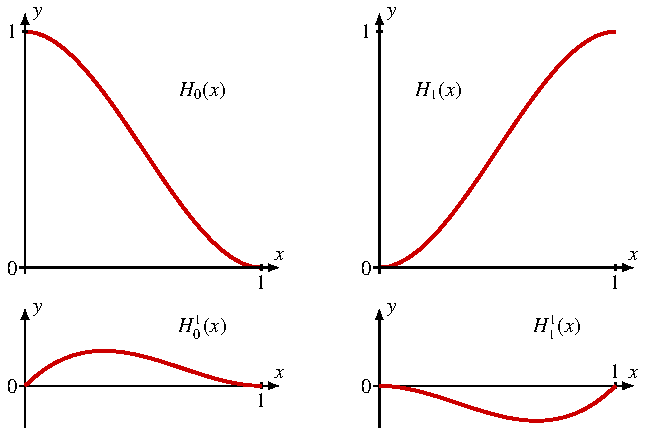
\includegraphics{chapters/030-nichtdiff/images/hermite.pdf}
\caption{Hermite-Polynome
\label{buch:nichtdiff:splines:fig:hermitepolynome}}
\end{figure}

Es müssen kubische Polynome auf dem Intervall $[x_k,x_{k+1}]$ konstruiert
werden, die vorgegebene Werte und Ableitungen in den Intervallenden haben.
Diese Aufgabe kann auf dem Intervall $[0,1]$ sofort gelöst werden,
wenn kubische Polynome auf dem bekannt sind, deren Werte der Funktion
und ersten Ableitungen an den Endpunkten $0$ sind mit Ausnahme jeweils eines,
der $1$ ist (Abbildung~\ref{buch:nichtdiff:splines:fig:hermitepolynome}).

\begin{satz}
\label{buch:nichtdiff:splines:satz:hermitebasis}
Die Polynome
\begin{align*}
H_0(x)   &=  (1+2x)(1-x)^2 = 2x^3-3x^2+1,
&&&
H_1(x)   &=      (3-2x)x^2 = -2x^3+3x^2,
\\
H_0^1(x) &=       x(1-x)^2 = x^3-2x^2+x,
&&\text{und}&
H_1^1(x) &=       (1-x)x^2 = x^3-x^2
\end{align*}
haben die Funktionswerte
\begin{align*}
H_0(0) &= 1,& H_1(0) &= 0,& H_0^1(0) &= 0,& H_0^1(1) &= 0,\\
H_0(1) &= 0,& H_1(1) &= 1,& H_0^1(0) &= 0,& H_0^1(1) &= 0
\intertext{und Werte der ersten Ableitungen}
H_0'(0) &= 0,& H_1'(0) &= 0,& H_0^{1\prime}(0) &= 1,& H_0^{1\prime}(1) &= 0,\\
H_0'(1) &= 0,& H_1'(1) &= 0,& H_0^{1\prime}(0) &= 0,& H_0^{1\prime}(1) &= 1
\end{align*}
an den Intervallenden.
Die zweiten Ableitungen der Polynome an den Intervallenden sind
\begin{align*}
H_0''(0) &= -6,& H_1''(0) &= \phantom{-}6,
&
H_0^{1\prime\prime}(0) &= -4,& H_1^{1\prime\prime}(0) &= -2,
\\
H_0''(1) &= \phantom{-}6 & H_1''(1) &= -6,
&
H_0^{1\prime\prime}(1) &=  \phantom{-}2,& H_1^{1\prime\prime}(1) &=  \phantom{-}4.
\end{align*}
\end{satz}

\begin{proof}
Die Behauptungen können durch Einsetzen der Argumente $0$ und $1$ in
die Polynome und ihre Ableitungen unmittelbar verifiziert werden.
\end{proof}

Mit den Polynomen von Satz~\ref{buch:nichtdiff:splines:satz:hermitebasis}
lässt sich die Aufgabe jetzt für ein Polynom auf einem Intervall
beliebiger Länge $l$ lösen.
Sei $P(x)$ ein kubisches Polynom.
Das Polynom $p(x)=P(x/l)$ ist ebenfalls kubisch und hat die Ableitungen
\[
p'(x) = P'(x/l)/l
\qquad\text{und}\qquad
p''(x) = P''(x/l)/l^2.
\]
Mit Hilfe einer Translation kann nun auch erreicht werden, dass die
verlangen Werten in den Punkten $x_k$ und $x_{k+1}$ angenommen werden.
Das Polynom
\(
p(x) = P((x-x_k)/(x_{k+1}-x_k))
\)
erfüllt
\begin{align*}
p(x_k)   &= P(0),                  &&          & p(x_{k+1})   &= P(1),               \\
p'(x_k)  &= P'(0)/(x_{k+1}-x_k),   &&          & p'(x_{k+1})  &= P'(1)/(x_{k+1}-x_k),\\
p''(x_k) &= P''(0)/(x_{k+1}-x_k)^2 &&\text{und}& p''(x_{k+1}) &= P''(1)/(x_{k+1}-x_k).
\end{align*}
Zur Vereinfachung der Notation bezeichnen wir die Länge der Teilintervalle
im Folgenden mit $m_k=x_{k+1}-x_k$.
Mit diesen Notation können wir jetzt für jedes Teilintervall $[x_k,x_{k+1}]$
ein kubisches Polynom konstruieren, welches die verlangten Werte und ersten
Ableitungen hat.

\begin{satz}
\label{buch:nichtdiff:splines:satz:polynom}
Das Polynom
\begin{equation}
y_k(x)
=
y_k
H_0\biggl(\frac{x-x_k}{m_k}\biggr)
+
y_{k+1}
H_1\biggl(\frac{x-x_k}{m_k}\biggr)
+
s_k
m_k
H_0^1\biggl(\frac{x-x_k}{m_k}\biggr)
+
s_{k+1}
m_{k}
H_1^1\biggl(\frac{x-x_k}{m_k}\biggr)
\label{buch:nichtdiff:splines:eqn:ykdarstellung}
\end{equation}
hat die Funktionswerte und ersten und zweiten Ableitungen
\begin{align*}
y_k(x_k)       &= y_k,
&
y_k'(x_k)      &= s_k,
&
y_k''(x_k)     &=
-\frac{6y_k}{m_k^2} + \frac{6y_{k+1}}{m_k^2}
-
\frac{4s_k}{m_k} - \frac{2s_{k+1}}{m_k},
\\
y_k(x_{k+1})   &= y_{k+1},
&
y_k'(x_k)      &= s_{k+1},
&
y_k''(x_{k+1}) &=
\phantom{-}\frac{6y_k}{m_k^2} - \frac{6y_{k+1}}{m_k^2}
+
\frac{2s_k}{m_k} + \frac{4s_{k+1}}{m_k}.
\end{align*}
\end{satz}

%
% Gleichungssystem für die Steigungen in den Stützstellen
%
\subsubsection{Gleichungssystem für die Steigungen in den Stützstellen}
Mit den im vorangegangenen Abschnitt gefundenen Polynome kann eine
Spline-Inter\-po\-la\-tions\-funktion konstruiert werden, sobald die ersten
Ableitungen der Funktion in den Stützstellen bekannt sind.
Diese müssen so gewählt werden, dass die daraus konstruierten
Polynome an den Stützstellen die gleichen zweiten Ableitungen haben.
In diesem Abschnitt soll ein Gleichungssystem hergeleitet werden, mit
denen diese ersten Ableitungen bestimmt werden können.

Seien $s_k=y'(x_k)$ die noch unbekannten Ableitungen in den Stützstellen.
Ausserdem sei $m_k = x_{k+1}-x_k$ die Länge des Intervalls $[x_k,x_{k+1}]$.
Die in Satz~\ref{buch:nichtdiff:splines:satz:polynom} konstruierten
Funktionen $y_k$ müssen in den Stützstellen die gleichen zweiten
Ableitungen haben, also
\[
y_{k-1}''(x_k) =  y_{k}''(x_k).
\]
Mit den Werten der zweiten Ableitung nach
Satz~\ref{buch:nichtdiff:splines:satz:polynom}
folgen jetzt die Gleichungen
\begin{align*}
\frac{6y_{k-1}}{m_{k-1}^2}
-
\frac{6y_{k}}{m_{k-1}^2}
+
\frac{2s_{k-1}}{m_{k-1}^2}
+
\frac{4s_k}{m_{k-1}^2}
&=
- \frac{6y_k}{m_k^2}
+
\frac{6y_{k+1}}{m_k^2}
-
\frac{4s_k}{m_k}
-
\frac{2s_{k+1}}{m_k}
\intertext{für $0<k<n$ und}
y''_0(x_0)
=
0
&=
-\frac{6y_0}{m_0^2}
+\frac{6y_1}{m_0^2}
-\frac{4s_0}{m_0}
-\frac{2s_1}{m_0}
\\
y''_n(x_n)
=
0
&=
\frac{6y_{n-1}}{m_{n-1}^2}
-
\frac{6y_n}{m_{n-1}^2}
+
\frac{2s_{n-1}}{m_{n-1}}
+
\frac{4s_n}{m_{n-1}}
\intertext{an den Intervallenden.
Bringen wir die unbekannten $s_k$ auf die linke Seite und alles
andere auf die rechte Seite erhalten wir}
\frac{2}{m_{k-1}}s_{k-1}
+
\biggl(
\frac{4}{m_{k-1}}
+
\frac{4}{m_k}
\biggr)s_{k-1}
+
\frac{2}{m_{k-1}^2}s_{k-1}
&=
-
\frac{6}{m_{k-1}^2}
y_{k-1}
+
\biggl(
\frac{6}{m_{k-1}^2}
-
\frac{6}{m_k^2}
\biggr)
y_k
+
\frac{6}{m_k^2}
y_{k+1}
\\
&=
\frac{6}{m_{k-1}^2}(y_k-y_{k-1})
+
\frac{6}{m_k^2}(y_{k+1}-y_k)
\intertext{für $0<k<n$ und}
\frac{4}{m_0}s_0
+
\frac{2}{m_0}s_1
&=
-\frac{6}{m_0^2}y_0
+\frac{6}{m_0^2}y_1
=
\frac{6}{m_0^2}(y_1-y_0)
\\
\frac{2}{m_{n-1}}s_{n-1}
+
\frac{4}{m_{n-1}}s_n
&=
-\frac{6}{m_{n-1}^2}y_{n-1}
+\frac{6}{m_{n-1}^2}y_n
=
\frac{6}{m_{n-1}^2}(y_n-y_{n-1})
\end{align*}
an den Intervallenden.
Dies ist ein lineares Gleichungssystem mit $n+1$ Gleichungen
für die $n+1$ Unbekannten $s_k$.
Wir schreiben es in Matrixform mit der Koeffizientenmatrix
\begin{equation}
\renewcommand{\arraystretch}{1.9}
A=
\begin{pmatrix}
\displaystyle\frac{2}{m_0}
	&\displaystyle\frac{1}{m_0}
		&
			&
				&
					&
\\
\displaystyle\frac{1}{m_0}
	&\displaystyle\frac{2}{m_0}+\frac{2}{m_1}
		&\displaystyle\frac{1}{m_1}
			&
				&
					&
\\
	&\displaystyle \frac{1}{m_1}
		&\displaystyle \frac{2}{m_1} + \frac{2}{m_2}
			&\displaystyle \frac{1}{m_2}
				&
					&
\\
	&
		&\displaystyle\frac{1}{m_2}
			&\ddots
				&\ddots
					&
\\
	&
		&
			&\ddots
				&\ddots
					&\displaystyle\frac{1}{m_{n-1}}
\\
	&
		&
			&
				&\displaystyle\frac{1}{m_{n-1}}
					&\displaystyle\frac{2}{m_{n-1}}
\end{pmatrix}
\label{buch:nichtdiff:splines:eqn:matrixA}
\end{equation}
und der rechten Seite
\begin{equation}
\renewcommand{\arraystretch}{1.9}
b
=
3
\begin{pmatrix}
\displaystyle
\frac{1}{m_0^2}(y_1-y_0)
\\
\displaystyle
\frac{1}{m_0^2}(y_1-y_0)
+
\frac{1}{m_1^2}(y_2-y_1)
\\
\displaystyle
\frac{1}{m_1^2}(y_2-y_1)
+
\frac{1}{m_2^2}(y_3-y_2)
\\
\vdots
\\
\displaystyle
\frac{1}{m_{n-2}^2}(y_{n-1}-y_{n-2})
+
\frac{1}{m_{n-1}^2}(y_n-y_{n-1})
\\
\displaystyle
\frac{1}{m_{n-1}^2}(y_n-y_{n-1})
\end{pmatrix}.
\label{buch:nichtdiff:splines:eqn:vektorb}
\end{equation}
Schreibt man die Ableitungen $s_k$ als Vektor $s$, können die Steigungen
durch Lösen der Gleichung
\begin{equation}
As=b
\label{buch:nichtdiff:splines:eqn:gleichungssystem}
\end{equation}
bestimmt werden.
Die spezielle {\em tridiagonale} Form der Matrix $A$
\index{tridiagonal}%
ermöglicht eine sehr effiziente Berechnung der Steigungen, den
Thomas-Algorithmus \cite{buch:thomas}.
\index{Thomas-Algorithmus}%
Sobald die Steigungen $s_k$ bestimmt sind, können die Funktionen
$y_k(x)$ mit Satz~\ref{buch:nichtdiff:splines:satz:polynom}
berechnet werden.

%
% Äquidistante Stützstellen
%
\subsubsection{Äquidistante Stützstellen}
Haben die Stützstellen gleichen Haben die Stützstellen Abstand, man
spricht von äquidistanten Stützstellen, dann sind alle $m_k$ gleich.
Wir schreiben $m=m_k$ für alle $k=0,\dots,n-1$.
In diesem Fall vereinfachen sich die Gleichungen beträchtlich, da
alle Nenner gleich sind.
Die Koeffizientenmatrix des Gleichungssystems ist
\[
A
=
\begin{pmatrix}
2 &1 &  &       &       &  \\
1 &4 &1 &       &       &  \\
  &1 &4 &1      &       &  \\[-3pt]
  &  &1 &\ddots &\ddots &  \\[-3pt]
  &  &  &\ddots &\ddots &1 \\
  &  &  &       &1      &2
\end{pmatrix}
\]
und die rechte Seite wird
\[
b
=
\frac{3}{m}
\begin{pmatrix}
y_1-y_0\\
y_2-y_0\\
y_3-y_1\\[-3pt]
\vdots\\
y_n-y_{n-2}\\
y_n-y_{n-1}
\end{pmatrix}
\]

\begin{beispiel}
\label{buch:nichtdiff:splines:bsp:sinspline}
%
% sinspline.tex -- template for standalon tikz images
%
% (c) 2021 Prof Dr Andreas Müller, OST Ostschweizer Fachhochschule
%
\documentclass[tikz]{standalone}
\usepackage{amsmath}
\usepackage{times}
\usepackage{txfonts}
\usepackage{pgfplots}
\usepackage{csvsimple}
\usetikzlibrary{arrows,intersections,math}
\definecolor{darkred}{rgb}{0.8,0,0}
\definecolor{darkgreen}{rgb}{0,0.6,0}
\begin{document}
\input{sinpath.tex}
\def\skala{1}
\begin{tikzpicture}[>=latex,thick,scale=\skala]

\draw[->] (-0.1,0) -- ({3*3.14159+0.4},0) coordinate[label={$x$}];
\draw[->] (0,-2.1) -- (0,7.6) coordinate[label={right:$y$}];

\draw (-0.05,6) -- (0.05,6);
\node at (-0.05,6) [left] {$1\mathstrut$};
\draw[line width=0.3pt] (0,6) -- ({3*3.14159},6);
\draw ({3*3.14159},-0.05) -- ({3*3.14159},0.05);
\node at ({3*3.14159},-0.05) [below] {$\displaystyle\frac{\pi}2$};
\node at (-0.05,0) [left] {$0\mathstrut$};

\draw[color=darkgreen] \fehlerspline;

\draw[color=orange] \fehlerhermite;

\draw[color=blue] plot[domain=0:90,samples=100]
	({6*3.14159*\x/180},{6*sin(\x)});

\draw[color=darkred,line width=1.4pt] \spline;

\foreach \x in {0,9,...,90}{
	\fill[color=blue,line width=1.4pt]
		({6*3.14159*\x/180},{6*sin(\x)}) circle[radius=0.08];
}

\end{tikzpicture}
\end{document}


%
% sinspline.tex -- template for standalon tikz images
%
% (c) 2021 Prof Dr Andreas Müller, OST Ostschweizer Fachhochschule
%
\documentclass[tikz]{standalone}
\usepackage{amsmath}
\usepackage{times}
\usepackage{txfonts}
\usepackage{pgfplots}
\usepackage{csvsimple}
\usetikzlibrary{arrows,intersections,math}
\definecolor{darkred}{rgb}{0.8,0,0}
\definecolor{darkgreen}{rgb}{0,0.6,0}
\begin{document}
\input{sinpath.tex}
\def\skala{1}
\begin{tikzpicture}[>=latex,thick,scale=\skala]

\draw[->] (-0.1,0) -- ({3*3.14159+0.4},0) coordinate[label={$x$}];
\draw[->] (0,-2.1) -- (0,7.6) coordinate[label={right:$y$}];

\draw (-0.05,6) -- (0.05,6);
\node at (-0.05,6) [left] {$1\mathstrut$};
\draw[line width=0.3pt] (0,6) -- ({3*3.14159},6);
\draw ({3*3.14159},-0.05) -- ({3*3.14159},0.05);
\node at ({3*3.14159},-0.05) [below] {$\displaystyle\frac{\pi}2$};
\node at (-0.05,0) [left] {$0\mathstrut$};

\draw[color=darkgreen] \fehlerspline;

\draw[color=orange] \fehlerhermite;

\draw[color=blue] plot[domain=0:90,samples=100]
	({6*3.14159*\x/180},{6*sin(\x)});

\draw[color=darkred,line width=1.4pt] \spline;

\foreach \x in {0,9,...,90}{
	\fill[color=blue,line width=1.4pt]
		({6*3.14159*\x/180},{6*sin(\x)}) circle[radius=0.08];
}

\end{tikzpicture}
\end{document}


Wir approximieren die Sinusfunktion $f(x)=\sin x$ mit Hilfe eines Splines
mit elf äquidistanten Stützstellen.
Die Stützstellen und Funktionswerte sind
\[
x_k = \frac{k\pi}{20}
\quad\text{und}\quad
y_k = \sin\frac{k\pi}{20}
\quad\text{für}\quad
k=0,\dots,10.
\]
Mit dem Gleichungssystem~\eqref{buch:nichtdiff:splines:eqn:gleichungssystem}
können die Steigungen $s_k$ berechnet werden, mit denen schliesslich die
Spline-Interpolationsfunktion berechnet werden kann.
Die Resultat sind in Tabelle~\ref{buch:nichtdiff:splines:table:sinspline}
zusammengestellt.
Abbildung~\ref{buch:nichtdiff:splines:fig:sinspline} zeigt den Unterschied
zwischen der Sinus-Funktion (blau) und der Spline-Interpolationsfunktion (rot),
es ist kaum ein Unterschied erkennbar.
Die Abweichung $y(x)-\sin x$ ist 1000-fach überhöht grün dargestellt, sie
ist vor allem am rechten Ende des Intervalls gross, wo die Krümmung grösser
ist.

Die Genauigkeit der Interpolation hängt vor allem von der Qualität der 
berechneten Steigungen $s_k$ ab.
Da diese im vorliegenden Fall exakt als $f'(x_k) = \cos x_k$ berechnet
werden können, kann man die Spline-Interpolationsfunktion mit der sogenannten
Hermite-Interpolationsfunktion vergleichen, die die wahren Steigungen
verwendet.
Die Abweichung zwischen der Sinus-Funktion und der
Hermite-Interpolationsfunktion ist 100000-fach überhöht orange dargestellt.
Bekannte Steigungen ermöglichen also eine viel höhere Genauigkeit, als dies
mit den geschätzten Steigungen möglich ist.
\end{beispiel}

%
% Finite Elemente auf einem Intervall
%
\subsubsection{Finite Elemente auf einem Intervall}
In Satz~\ref{buch:nichtdiff:splines:satz:hermitebasis} konzentrierte sich
die Aufmerksamkeit auf das Innere eines der Intervalle
$[x_{k\mathstrut},x_{k+1\mathstrut}]$.
Die Matrix $A$ von
\eqref{buch:nichtdiff:splines:eqn:matrixA}
und der Vektor $b$ von
\eqref{buch:nichtdiff:splines:eqn:vektorb}
lieferten dann die Koeffizienten für die Linearkombination der
auf diesem Intervall definierten Polynome
\[
H_0\biggl(\frac{x-x_k}{m_k}\biggr),
\qquad
H_1\biggl(\frac{x-x_k}{m_k}\biggr),
\qquad
H_0^1\biggl(\frac{x-x_k}{m_k}\biggr)
\qquad\text{und}\qquad
H_1^1\biggl(\frac{x-x_k}{m_k}\biggr),
\]
die das Interpolationspolynom $y_k(x)$ ergaben.
Sie heissen auch die {\em Formfunktionen}.
\index{Formfunktion}%

Jeder Wert $y_k$ und jede Steigung $m_k$ kam in der Darstellung
\eqref{buch:nichtdiff:splines:eqn:ykdarstellung} 
der beiden Funktionen $y_{k-1}(x)$ und $y_{k\mathstrut}(x)$ vor.
Fügt man diese Funktionen auf dem ganzen Intervall zusammen,
dann kann man die Interpolationsfunktion als Linearkombination
von auf $[a,b]$ definierten, stetig differenzierbaren Funktionen
schreiben, wobei die $y_k$ und $m_k$ die Koeffizienten sind.

%
% interpolation.tex
%
% (c) 2024 Prof Dr Andreas Müller
%
\begin{figure}
\centering
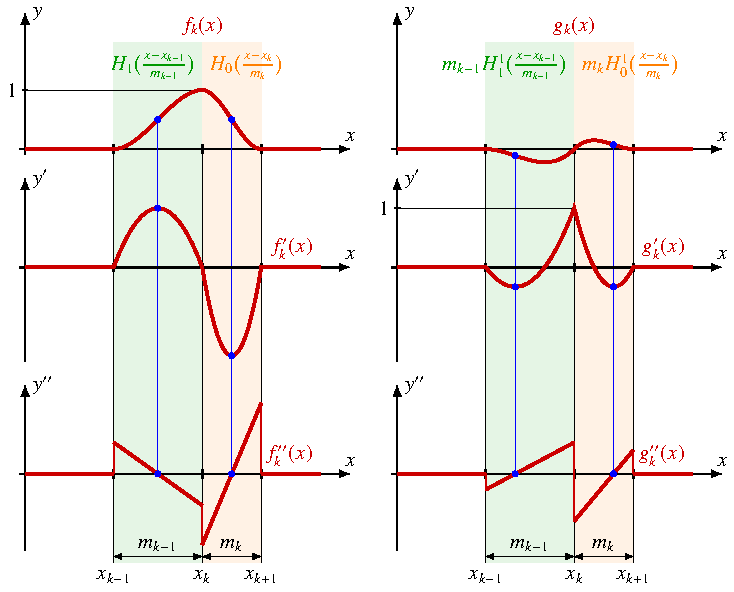
\includegraphics{chapters/030-nichtdiff/images/interpolation.pdf}
\caption{Basisfunktionen für die Spline-Interpolationsfunktion.
Die Spline-Interpolationsfunktion $y(x)$ ist Linearkombination der
Funktion $f_k(x)$, die nur an der Stützstellen $x_k$ den von Null
verschiedenen Wert $1$ und an allen Stützstellen verschwindende
Ableitung haben, und den Funktionen $g_k(x)$, deren Funktionswerte
an den Stützstellen verschwinden und deren Ableitungen nur an der
Stützstelle $x_k$ den von 0 verschiedenen Wert $1$ haben.
Die zweiten Ableitungen von $f_k(x)$ und $g_k(x)$ sind nicht
mehr stetig.
\label{buch:nichtdiff:splines:fig:interpolation}}
\end{figure}


\begin{satz}
Die Spline-Interpolationsfunktion ist die Linearkombination
\begin{equation}
y(x)
=
\sum_{k=0}^n y_k f_k(x)
+
\sum_{k=0}^n m_k g_k(x)
\label{buch:nichtdiff:spline:eqn:linearkomb}
\end{equation}
der Funktionen
\[
f_k(x)
=
\begin{cases}
\displaystyle
\phantom{m_{k-1\mathstrut}}
H_1\biggl(\frac{x-x_{k-1\mathstrut}}{m_{k-1\mathstrut}}\biggr)
	&\quad x\in[x_{k-1\mathstrut},x_{k\mathstrut}]\\[5pt]
\displaystyle
\phantom{m_{k-1\mathstrut}}
H_0\biggl(\frac{x-x_{k\mathstrut}}{m_{k\mathstrut}}\biggr)
	&\quad x\in[x_{k\mathstrut},x_{k+1\mathstrut}]\\
\phantom{m_{k-1\mathstrut}}
0&\quad\text{sonst}
\end{cases}
\]
und
\[
g_k(x)
=
\begin{cases}
\displaystyle
m_{k-1\mathstrut}
H_1^1\biggl(\frac{x-x_{k-1\mathstrut}}{m_{k-1\mathstrut}}\biggr)
	&\quad x\in[x_{k-1\mathstrut},x_{k\mathstrut}]\\[5pt]
\displaystyle
\phantom{m_{k-1\mathstrut}}\llap{$m_k\mathstrut$}
H_0^1\biggl(\frac{x-x_{k\mathstrut}}{m_{k\mathstrut}}\biggr)
	&\quad x\in[x_{k\mathstrut},x_{k+1\mathstrut}]\\
\phantom{m_{k-1\mathstrut}}
0&\quad\text{sonst,}
\end{cases}
\]
die auf dem ganzen Intervall stetig differenzierbar sind.
\end{satz}

Die Funktionen $f_k(x)$ und $g_k(x)$ sind in
Abbildung~\ref{buch:nichtdiff:splines:fig:interpolation}
dargestellt.
Die Funktion $f_k(x)$ verschwindet an allen Stützstellen ausser
an der Stützstelle $x_k$, wo sie den Wert $1$ hat.
Die Ableitung von $f_k(x)$ verschwindet ebenfalls in allen Stützstellen.
Die Funktion $g_k(x)$ verschwindet in allen Sütztstellen.
Auch verschwinden alle Ihre Ableitungen ausser in der Stützstelle $x_k$,
wo $g_k'(x_k)=1$ ist.

\begin{proof}
Es ist zunächst zu prüfen, ob Linearkombination
\eqref{buch:nichtdiff:spline:eqn:linearkomb},
die wir für die Zwecke des Beweises mit $l(x)$ bezeichnen wollen,
auf dem Teilintervall $[x_{k\mathstrut},x_{k+1\mathstrut}]$
die Spline-Interpolationsfunktion ergibt.
Dazu beachtet man, dass der Träger der Funktionen $f_k(x)$ und $g_k(x)$ 
das Intervall $[x_{k-1\mathstrut},x_{k+1\mathstrut}]$ ist.
Auf dem Teilintervall $[x_{k\mathstrut},x_{k+1\mathstrut}]$ sind von
den Funktionen $f_l$ und $g_l$ genau die vier Funktion $f_{k\mathstrut}$,
$g_{k\mathstrut}$, $f_{k+1\mathstrut}$ und $g_{k+1\mathstrut}$
von $0$ verschieden.
Auf dem Intervall $[x_{k\mathstrut},x_{k+1\mathstrut}]$ ist daher die
Linearkombination~\eqref{buch:nichtdiff:spline:eqn:linearkomb}
\begin{align*}
l(x)
&=
y_{k\mathstrut}
f_{k\mathstrut}(x)
+
y_{k+1\mathstrut}
f_{k+1\mathstrut}(x)
+
s_{k\mathstrut}
g_{k\mathstrut}(x)
+
s_{k+1\mathstrut}
g_{k+1\mathstrut}(x).
\intertext{Ersetzen wir die Funktionen durch ihre Definition auf dem
Teilintervall $[x_{k\mathstrut},x_{k+1\mathstrut}]$, wird daraus}
&=
y_{k\mathstrut}
H_0\biggl(\frac{x-x_{k\mathstrut}}{m_{k\mathstrut}}\biggr)
+
y_{k+1\mathstrut}
H_1\biggl(\frac{x-x_{k\mathstrut}}{m_{k\mathstrut}}\biggr)
+
s_{k\mathstrut}
m_{k\mathstrut}
H_0^1\biggl(\frac{x-x_{k\mathstrut}}{m_{k\mathstrut}}\biggr)
+
s_{k+1\mathstrut}
m_{k\mathstrut}
H_1^1\biggl(\frac{x-x_{k\mathstrut}}{m_{k\mathstrut}}\biggr).
\end{align*}
Dies stimmt mit der Darstellung
\eqref{buch:nichtdiff:splines:eqn:ykdarstellung}
von Satz~\ref{buch:nichtdiff:splines:satz:polynom}
überein.
Damit ist gezeigt, dass die Linearkombination $l(x)$ die 
Spline-Interpolationsfunktion $y(x)$ ist, $y(x)=l(x)$.

Als Polynome sind die Funktionen $f_k(x)$ und $g_k(x)$ im Inneren der
aller Intervalle $[x_{i\mathstrut},x_{i+1\mathstrut}]$ stetig
differenzierbar, es ist also nur noch zu prüfen, ob die Ableitungen
der Teilfunktionen in den Stützstellen $x_{k-1\mathstrut}$, $x_{k\mathstrut}$
und $x_{k+1\mathstrut}$ übereinstimmen.
Die Ableitung von $f_k(x)$ ist
\[
f_k'(x)
=
\begin{cases}
\displaystyle
\frac{1}{m_{k-1\mathstrut}}
H'_1\biggl(\frac{x-x_{k-1\mathstrut}}{m_{k-1\mathstrut}}\biggr)
&\qquad x \in [x_{k-1\mathstrut},x_{k\mathstrut}]\\
\displaystyle
\phantom{\frac{1}{m_{k-1\mathstrut}}}
\llap{$\displaystyle\frac{1}{m_{k\mathstrut}}$}
H'_0\biggl(\frac{x-x_{k\mathstrut}}{m_{k\mathstrut}}\biggr)
&\qquad x \in [x_{k\mathstrut},x_{k+1\mathstrut}]\\
\phantom{\displaystyle\frac{1}{m_{k-1\mathstrut}}}
0&\qquad\text{sonst.}
\end{cases}
\]
Die Ableitungen $H_0'(x)$ und $H_1'(x)$ verschwinden aber in den Intervallenden
und somit sind auch die Ableitungen $f'_k(x_i)=0$ für alle Stützstellen $x_i$.
Die Ableitung von $g_k(x)$ ist
\[
g'_k(x)
=
\begin{cases}
\displaystyle
\phantom{m_{k-1}}
H_1^{1\prime}\biggl(\frac{x-x_{k-1\mathstrut}}{m_{k-1\mathstrut}}\biggr)
&\qquad x\in[x_{k-1\mathstrut},x_{k\mathstrut}]\\
\displaystyle
\phantom{m_{k-1}}
H_0^{1\prime}\biggl(\frac{x-x_{k\mathstrut}}{m_{k\mathstrut}}\biggr)
&\qquad x\in[x_{k\mathstrut},x_{k+1\mathstrut}]\\
\displaystyle
\phantom{m_{k-1}}
0
&\qquad\text{sonst.}
\end{cases}
\]
In den Stützstellen $x_{k-1}$ und $x_{k+1}$ verschwinden die Ableitungen
der Teilfunktionen.
In der Stützstelle $x_k$ gilt
\begin{align*}
g_k'(x_k-)
&=
H_1^{\prime 1}\biggl(
\frac{x_{k\mathstrut}-x_{k-1\mathstrut}}{m_{k-1\mathstrut}}
\biggr)
=
H_1^{\prime 1}(1)
=
1
\\
g_k'(x_k+)
&=
H_0^{\prime 1}\biggl(
\frac{x_{k\mathstrut}-x_{k\mathstrut}}{m_{k\mathstrut}}
\biggr)
=
H_0^{\prime 1}(0)
=
1,
\end{align*}
die Ableitungen der Teilfunktionen stimmen also überein.
\end{proof}


%
% Fehlerformel
%
%\subsubsection{Fehlerformel}

